\documentclass{article}

\usepackage{incertia}
\usepackage{stmaryrd}
\usepackage{tikz-cd}
\usetikzlibrary{arrows}

% setup the header
\pagestyle{fancy}
\lhead{Will Song}
\chead{Math 427}
\rhead{\today}


\title{Math 427 Notes}
\author{Will Song}
\date{Fall 2015}

\begin{document}

\maketitle
\newpage

\tableofcontents
\newpage

\section{Day 1 - Well Ordering}

\begin{prop}
Well ordering implies induction.
\end{prop}

\begin{proof}
Take $S \subseteq \mathbb{N}$ such that $1 \in S$ and $n + 1 \in S$ if
$n \in S$. Suppose for the sake of contradiction that $S \neq
\mathbb{N}$. Consider $S' = S \setminus \mathbb{N}$. By well ordering,
$S'$ has minimal element $m \neq 1$ due to $1 \in S$, so $m - 1 \in S$
by set difference. But then $m \in S$ by assumption on $S$ so $m \not
\in S'$ so $S'$ has no minimal element which contradicts well ordering.
\end{proof}

\begin{prop}
Induction implies well ordering
\end{prop}

\begin{proof}
Suppose $S \subseteq \mathbb{N}, S \neq \varnothing$.

Suppose that $S$ has no smallest element. Then $1 \not \in S$ because
$1$ is the minimal element of $\mathbb{N}$ and thus $S$. Suppose $1, 2,
3, \dots, k \not \in S$, then $k + 1 \not \in S$ because it would then be
the smallest element in $S$. Then $n \not \in S \forall n \in
\mathbb{N}$, so $S = \varnothing$.
\end{proof}

\begin{prop}
For any $a, d \in \mathbb{Z}, d \neq 0$, then we can write $a = qd + r,
0 \leq r < d$ with $q, d$ unique.
\end{prop}

\begin{proof}
% cheating
$ $\newline
\textbf{Existence}: Consider the set $S = \lbrace x = a - qd \mid x
\geq 0 \rbrace$. At least one of $a$, $-a$ is in $S$ so $S$ is non-empty
and has a minimal element by well ordering. We take $r = \min S$ and $q$
to be the corresponding $r = a - qd$. If $r \not < d$, then $r - d = a -
(q + 1)d \in S$ which contradicts the minimality of $r$, so we are done
(for existence).

\textbf{Uniqueness}: Let $a = q_1 d + r_1 = q_2 d + r_2$. Then $0 = a -
a = (q_1 - q_2) d + (r_1 - r_2)$, or $q_1 - q_2 = 0, r_1 - r_2 = 0$
because of restrictions on $r_1, r_2$.
\end{proof}

\section{Day 2}

\subsection{Cylindrical Coordinates}
\begin{center}
\begin{asy}
import three;
import graph3;

settings.render = 0;
settings.prc = false;

size(8cm);

currentprojection = perspective(5, 1, 3.5);

real z = 4;
triple p  = (0, 0, z);
triple q  = (1, sqrt(3), z);
triple x  = (1, sqrt(3), 0);
triple ap = point(O -- x, 0.3);
triple aq = rotate(-60, Z) * ap;
//path c = 2X .. 2Y .. -2X .. -2Y .. cycle;

draw(L = Label("$x$", position = Relative(1.1), align = SW), O -- 5 X,
red + 0.75, Arrow3);
draw(L = Label("$y$", position = Relative(1.1), align = SE), O -- 5 Y,
blue + 0.75, Arrow3);
draw(L = Label("$z$", position = Relative(1.1), align =  N), O -- 6 Z,
green + 0.75, Arrow3);

draw(L = Label("$\vec{s}$", position = Relative(0.5), align = N), p --
q, Arrow3);
draw(L = Label("$\vec{r}$", position = Relative(0.5), align = E), O --
q, Arrow3);

draw(O -- x);
draw(L = Label("$z$", position = Relative(0.5), align = E), q -- x, dashed);
draw(L = Label("$\phi$", position = Relative(0.5), align = (0.0005,
-0.0005)), arc(O, ap, aq));

draw(2X .. 2Y .. -2X .. -2Y .. cycle, dashed);
draw(2X + z * Z .. 2Y + z * Z .. -2X + z * Z .. -2Y + z * Z .. cycle,
dashed);

//draw(rotate(180, Z) * q -- rotate(180, Z) * x, dashed);

dot(q);

label("$P = (s, \phi, z)$", q, SE);
\end{asy}
\end{center}

We have the coordinates $(s, \phi, z)$ where $s$ is the distance from
the vertical axis, $\phi$ is the rotational angle with respect to the
plane perpendicular to the vertical axis, and $z$ is the position on the
vertical axis. This gives us a nice definition for the position vector.
\[ \vec{r} = s \hat{s} + z \hat{z} \]

\begin{note}
The unit vectors $\hat{s}, \hat{\phi}$ are position dependent! More
specifically, they depend on $\phi$.

We have
\[ \frac{\partial \hat{s}}{\partial \phi} = \hat{\phi} \quad
\frac{\partial \hat{\phi}}{\partial \phi} = -\hat{s}. \]
\end{note}

\begin{cor}
We then have the line element
\[ d \vec{r} = d \vec{l} = \left( \frac{\partial}{\partial s} ds +
\frac{\partial}{\partial \phi} d \phi + \frac{\partial}{\partial z} dz
\right) \vec{r} = ds \hat{s} + s d \phi \hat{\phi} + dz \hat{z}, \]
% \[ d \vec{r} = d \vec{l} = d(s \hat{s} + z \hat{z}), \]
velocity
\[ \vec{v} = \frac{d \vec{r}}{dt} = \frac{ds}{dt} \hat{s} + s \frac{d
\phi}{dt} \hat{\phi} + \frac{dz}{dt} \hat{z} = \dot{s} \hat{s} + s
\dot{\phi} \hat{\phi} + \dot{z} \hat{z}, \]
and acceleration
\[ \begin{aligned}
\vec{a} = \frac{d \vec{v}}{dt} &= \frac{d}{dt} \left( \dot{s} \hat{s}
+ s \dot{\phi} \hat{\phi} + \dot{z} \hat{z} \right) \\
&= \ddot{s} \hat{s} + \dot{s} \frac{d \hat{s}}{dt}  + \dot{s} \dot{\phi}
\hat{\phi} + s \ddot{\phi} \hat{\phi} + s \dot{\phi} \frac{d
\hat{\phi}}{dt} + \ddot{z} \hat{z} + \dot{z} \frac{d \hat{z}}{dt} \quad
\textrm{(product rule rocks)} \\
&= \ddot{s} \hat{s} + \dot{s} \frac{d \hat{s}}{d \phi}\frac{d \phi}{dt}
+ \dot{s} \dot{\phi} \hat{\phi} + s \ddot{\phi} \hat{\phi} + s
\dot{\phi} \frac{d \hat{\phi}}{d \phi} \frac{d \phi}{dt} + \ddot{z}
\hat{z} \\
&= \ddot{s} \hat{s} + \dot{s} \hat{\phi} \dot{\phi} + \dot{s} \dot{\phi}
\hat{\phi} + s \ddot{\phi} \hat{\phi} - s \dot{\phi} \hat{s} \dot{\phi}
+ \ddot{z} \hat{z} \\
&= \left( \ddot{s} - s \dot{\phi}^2 \right) \hat{s} + \left( s
\ddot{\phi} + 2 \dot{s} \dot{\phi} \right) \hat{\phi} + \ddot{z} \hat{z}
\end{aligned} \]
\end{cor}

\begin{rem}
Notice here that $d \hat{s}$ refers to the total differential of
$\hat{s}$, as well as $d \hat{\phi}$ and $d \hat{z}$. Where total
differential of a function $f : \mathbb{R} \times \mathbb{R} \times
\cdots \times \mathbb{R} \to \mathbb{R}$ is defined as
\[ df(x_1, x_2, \dots, x_n) = \left( \sum_{i = 1}^n
\frac{\partial}{\partial x_i} d x_i \right) f. \]
\end{rem}

\begin{ex}
We have a trajectory
\[ \begin{aligned}
s(t) &= R, \\
\phi(t) &= \omega t, \\
z(t) &= \alpha t. \\
\end{aligned} \]
Compute $|\vec{v}(t)|$ and $\vec{a}$.
\end{ex}

\begin{proof}[Solution]
We simply plug.
\[ \begin{aligned}
\vec{v} &= \dot{s} \hat{s} + s \dot{\phi} \hat{\phi} + \dot{z} \hat{z}
\\
&= 0 \hat{s} + R \omega \hat{\phi} + \alpha \hat{z} \\
&\Downarrow \\
\Aboxed{|\vec{v}| &= \sqrt{R^2 \omega^2 + \alpha^2}} \\
\vec{a} &= (0 - R \omega^2) \hat{s} + (0 + 0) \hat{\phi} + 0 \hat{z} \\
\Aboxed{ &= -R \omega^2 \hat{s}.}
\end{aligned} \]

Notice how this makes sense because $a = \frac{v^2}{r} = \frac{R^2
\omega^2}{R}$
\end{proof}

\begin{ex}
Consider a mass of mass $m$ swinging on a rope of length $R$ with normal
gravity $g$. Assuming no friction, determine $\phi(t)$ where $\phi$
represents the angle from rest of the mass.

\begin{center}
\begin{asy}
size(6cm);

pair O = (0, 0);
pair P = (-1, -sqrt(3));

draw(arc(O, 2, 210, 330), Arrows);
draw("$R$", O -- P);
draw(O -- (0, -2), dashed);

draw("$\phi$", arc(O, 0.3, 240, 270));
draw("$g$", P -- (P + 0.8S), right, Arrow);

dot(O);
dot(P);

label("$m$", P, SW);
\end{asy}
\end{center}
\end{ex}

\begin{proof}[Solution]
Again we will refer back to the glorious equation $\vec{F} = m
\ddot{\vec{r}}$. Luckily $z = 0$ so we can leave that out of our
calculations.

\[ \vec{F} = mg(\cos \phi \hat{s} - \sin \phi \hat{\phi}) + \vec{F}_N \]
but $\vec{F}_N$ is such that $\frac{ds}{dt} = 0$ so we end up with
\[ \vec{F} = -mg \sin \phi \hat{\phi} = m \ddot{\vec{r}} \implies
\ddot{\vec{r}} = -g \sin \phi \hat{\phi}, \]
which we can rewrite as
\[ \left(s \ddot{\phi} + 2 \dot{s} \dot{\phi} \right) \hat{\phi} = -g
\sin \phi \hat{\phi} \implies \ddot{\phi} = -\frac{g}{s} \sin \phi, \]
which does not have a very nice solution, but we can approximate $\sin
\phi \approx \phi$ for small $\phi$, so this becomes $\ddot{\phi} =
-\frac{g}{s} \phi$, which has the nice solution
\[ \phi(t) = \alpha \sin\left( \sqrt{\frac{g}{s}} t + \psi \right) \]
for some optimal choice of $\psi$ and $\alpha = \max \phi$.
\end{proof}

\section{Day 3}

\subsection{Notes on Homework 1}
Learn how to do math. For example $1 - x^2 = (1 + x)(1 - x)$. Also trig
is nice.
\[ \begin{aligned}
\sin (A + B) &= \sin A \cos B + \cos A \sin B \\
\cos (A + B) &= \cos A \cos B + \sin A \sin B \\
\end{aligned} \]
Please use $\vec{F} = m \vec{a}$. Don't be stupid.

\subsection{Things}
Most of the time was spent covering the final example from
section~\ref{cylindrical}, which is kept in section~\ref{cylindrical}.

\subsection{2 Second Problems}
\begin{prb}[Triangle Inequality]
Show that $|\vec{a} + \vec{b}| \leq a + b$.
\end{prb}
\begin{proof}[Solution]
Expand.
\[ a^2 + b^2 + 2ab\cos\theta \leq a^2 + b^2 + 2ab. \]
\end{proof}

\begin{prb}
Evaluate
\[ \frac{d}{dt}\left(\vec{a} \cdot \left( \vec{v} \times \vec{r} \right)
\right). \]
\end{prb}
\begin{proof}[Solution]
Use product rule.
\[ \dot{\vec{a}} \cdot \left(\vec{v} \times \vec{r}\right)  + \vec{a}
\cdot \left(\vec{a} \times \vec{r}\right) + \vec{a} \cdot \left(\vec{v}
\times \vec{v}\right) = \dot{\vec{a}} \cdot \left(\vec{v} \times \vec{r}
\right). \]
\end{proof}

\begin{prb}
Consider $\vec{F} = F(x) \hat{x}$. Solve $F(x) = ma = m \ddot{x}$.
\end{prb}
\begin{proof}[Solution]
Write
\[ \begin{aligned}
F(x) &= ma = m \frac{dv}{dt} = m \frac{dx}{dt} \frac{dv}{dx} \\
\implies F(x) dx &= mv dv \\
\int_{x_0}^x F(u) du &= \frac{1}{2} m(v^2 - v_0^2) \\
v &= \sqrt{\frac{2}m \int_{x_0}^x F(u) du + v_0^2} \\
x &= \int_{t_0}^t \sqrt{\frac{2}m \int_{x_0}^x F(u) du + v_0^2} ds \\
\end{aligned} \]
and pray.
\end{proof}

\begin{prb}
Consider a bead located on a circular hoop of radius $R$ aligned with
the $z$ axis rotating with angular velocity $\omega$.
\end{prb}

\begin{proof}[Solution]
Here we have $\phi = \omega t + \phi_0, \dot{\phi} = \omega$. We have
$\vec{F}_g = -g\hat{z}, \vec{F}_s = -mR \omega^2 \hat{s}, \vec{F}_\theta
= -mR \dot{\theta}^2 \hat{r}$.

We also have $F_\theta = \sin \theta (r \ddot{\phi} + 2 \dot{r}
\dot{\phi}) + \cos \theta (2 r \dot{\theta} \dot{\phi})$, but
$\ddot{\phi} = 0, \dot{r} = 0$ so $F_\theta = 2 R \omega \dot{\theta}
\cos \theta$.
\end{proof}

\section{Day 4}

\begin{df}
A \textbf{relation} $R$ on a set $X$ is a subset $R \subseteq X \times
X$ and is written $x \, R \, y \Leftrightarrow (x, y) \in R$.
\end{df}

\begin{df}
A relation $\sim \, \subseteq X \times X$ is an \textbf{equivalence
relation} iff
\[ \begin{aligned}
x \in X &\implies x \sim x \\
x \sim y &\implies y \sim x \quad \forall x, y \in X \\
x \sim y, y \sim z &\implies x \sim z \quad \forall x, y, z \in X \\
\end{aligned} \]
\end{df}

\begin{df}
A \textbf{partition} of a set $x$ is a collection of subsets
$\mathcal{C}_{\alpha \in A} \in \mathcal{P}(X)$ such that
\[ \begin{aligned}
X &= \bigcup_{\alpha \in A} \mathcal{C}_\alpha \\
\mathcal{C}_\alpha \cap \mathcal{C}_\beta \neq \varnothing &\implies
\mathcal{C}_\alpha = \mathcal{C}_\beta \\
\end{aligned} \]
\end{df}

\begin{df}
Let $\sim$ be an equivalence relation on a set $X$. Then the equivalence
class of $x \in X$ is the set
\[ [x] = \lbrace y \in X : x \sim y \rbrace \]
\end{df}

\begin{thm}
Let $\sim$ be an equivalence relation on a non-empty set $X$. Then
\begin{enumerate}
\item The set of equivalence classes form a partition on $X$.
\item Any partition of $X$ defines an equivalence relation on $X$.
\end{enumerate}
\end{thm}

\begin{proof}
$ $\\
\begin{enumerate}
\item We have
\[ x \sim x \implies x \in [x] \implies X = \bigcup_{x \in X} [x]. \]
Now suppose $[x] \cap [y] \neq \varnothing$, which means $\exists z \in
X : z \in [x], z \in [y]$. Now take some representative element $w \in
[x]$ and write $z \sim x, w \sim x \implies w \sim z$. Now $z \in [y]$
so $z \sim y$, so $w \sim y \implies w \in [y]$, implying $[x] \subseteq
[y]$. Similarly, $[y] \subseteq [x]$ so $[x] = [y]$, finishing the proof
that the equivalence classes of $\sim$ form a partition on $X$.

\item For the other half, suppose we have a partition
$\mathcal{C}_{\alpha \in A}$. This implies that $\forall x \in X$,
$\exists \alpha \st x \in \mathcal{C}_\alpha$, which implies $x \sim x$.
If $x \sim y$, then $x, y \in \mathcal{C}_\alpha$ for some $\alpha$ so
$y \sim x$ as well. If $x, y \in \mathcal{C}_\alpha, y, z \in
\mathcal{C}_\beta$, then $\mathcal{C}_\alpha \cap \mathcal{C}_\beta \neq
\varnothing \implies x, y, z \in \mathcal{C}_\alpha = \mathcal{C}_\beta
\implies x \sim z$, which finishes the proof.
\end{enumerate}
\end{proof}

\begin{ex}
Take the relation $a \sim_n b \Leftrightarrow n \mid a - b, \quad a, b
\in \ZZ, n \in \NN$. Then $\sim_n$ is an equivalece relation on $\ZZ$.
\end{ex}

\begin{df}
The set of equivalence classes modulo $n$ are denoted $\ZZ/n\ZZ =
\lbrace [0], [1], \dots, [n - 1] \rbrace$ with a fairly standard
surjection $\pi : \ZZ \surj \ZZ/n\ZZ$ given by $a \mapsto [a]$.
\end{df}

\begin{thm}
$\ZZ/n\ZZ$ is a commutative ring with the usual operations $[a] + [b] =
[a + b]$ and $[a] \cdot [b] = [a \cdot b]$.
\end{thm}

\begin{proof}
Standard.
\end{proof}

\section{Day 5}

\subsection{Review}
Last time, we proved that equivalence relation $\Leftrightarrow$
partitions. However, we did not prove that the two implicit maps used in
the proof of \ref{eqpart} are inverses of each other.

We also got that the operations
\[ \begin{aligned}
+ : \ZZ/n\ZZ \times \ZZ/n\ZZ &\to \ZZ/n\ZZ \\
([a], [b]) &\mapsto [a + b] \\
* : \ZZ/n\ZZ \times \ZZ/n\ZZ &\to \ZZ/n\ZZ \\
([a], [b]) &\mapsto [a \cdot b] \\
\end{aligned} \]
are well defined.

\subsection{Groups}
\begin{df}
\label{binop}
A \textbf{binary operation} $\star$ on a set $S$ is a map $\star : S
\times S \to S$ which is often notated $a \star b := \star(a, b)$.
\end{df}

\begin{df}
\label{assoc}
A binary operation $\star$ is \textbf{associative} if $a \star (b \star
c) = (a \star b) \star c$.
\end{df}

\begin{df}
\label{commute}
A binary operation $\star$ is \textbf{commutative} if $a \star b = b
\star a$.
\end{df}

\begin{df}
\label{group}
A \textbf{group} is a set $G$ together with a binary operation $* : G
\times G \to G$, usually notated $(G, *)$, and a distinguished element
$e \in G$ such that
\begin{enumerate}
\item $*$ is associative.
\item $e * a = a = a * e \quad \forall a \in G$.
\item $\forall a \in g, \exists b \in G \st a * b = e = b * a$.
\end{enumerate}
\end{df}

\begin{prop}
In any group, inverses are unique.
\end{prop}

\begin{proof}
Suppose $b, c$ are inverses of $a$. Compute
\[ b = e * b = (c * a) * b = c * (a * b) = c * e = c. \]
\end{proof}

\begin{cor}
We can define a function $\operatorname{inv} : G \to G$ such that $g *
\operatorname{inv}(g) = e$. This is normally denoted $-a$ when the
operation is $+$ and $a^{-1}$ otherwise.
\end{cor}

\begin{df}
Define $GL_n(F) := \lbrace A \in M_n(F) : \det(A) \neq 0 \rbrace$ as the
set of invertible $n \times n$ matrices over $F$.
\end{df}

\begin{prop}
$GL_n(\RR)$ is a group with the usual multiplication.
\end{prop}

\section{Day 6}

\begin{df}
A group is said to be commutative or \textbf{abelian} if the operation
commutes.
\end{df}

\begin{ex}
Let $X$ be a set. Then the set of automorphisms $\aut(X) = \lbrace f : X
\to X \mid f \textrm{ invertible} \rbrace$ is a group under composition.
\end{ex}

\begin{prop}
$(a^{-1})^{-1} = a$.
\end{prop}

\begin{proof}
$a^{-1} * a = e$.
\end{proof}

\begin{df}
Let $G, H$ be two groups. A map $\varphi : G \to H$ is called a
\textbf{group homomorphism} iff $\varphi(a * b) = \varphi(a) *
\varphi(b) \quad \forall a, b \in G$.
\end{df}

\begin{ex}
We have the homomorphism from $\RR$ under $+$ to $\RR^*$ under $\cdot$
by $\exp(x) = e^x$.
\end{ex}

\begin{ex}
$\det : GL_n(F) \to F^*$ is a homomorphism.
\end{ex}

\begin{df}
Define the identity map on a set $X$ to be $\id_X : X \to X$ given by $x
\mapsto x$.
\end{df}

\begin{df}
A homomorphism $\varphi : G \to H$ is an \textbf{isomorphism} if there
is an inverse $\psi : H \to G$ such that $\varphi \circ \psi = \id_G,
\psi \circ \varphi = \id_H$.
\end{df}

\begin{prop}
Let $\varphi : G \to H$ be a bijective homomorphism. Then $\varphi^{-1}
: H \to G$ is a homomorphism.
\end{prop}

\begin{proof}
We want $\varphi^{-1}(xy) = \varphi^{-1}(x) \varphi^{-1}(y)$. Take
\[ \varphi(\varphi^{-1}(x) \varphi^{-1}(y)) = \varphi(\varphi^{-1}(x))
\varphi(\varphi^{-1}(y)) = xy = \varphi(\varphi^{-1}(xy)). \]
Injectivity on $\varphi$ gives the desired result.
\end{proof}

\begin{ex}
$\ln : (0, \infty) \to \RR^+$ has the inverse $\exp : \RR \to (0,
\infty)$.
\end{ex}

\section{Day 7 - New Things}

\begin{df}
A non-empty subset $H$ of a group $G$ is called a \textbf{subgroup} of
$G$ if $H$ is a group with respect to the binary operation of $G$.
\end{df}

\begin{ex}
$\ZZ$ is a subgroup of $\RR$ under $+$.
\end{ex}

\begin{rem}
If $H$ is a subgroup of $G$, then $e \in H$.
\end{rem}

\begin{rem}
The inclusion map $i : H \to G, i : h \mapsto h$ is a homomorphism.
\end{rem}

\begin{prop}
\label{subgroupcriteria}
Let $H \subseteq G$ and $H \neq \varnothing$. Then $H$ is a subgroup iff
$\forall h_1, h_2 \in H$, $h_1 h_2^{-1} \in H$.
\end{prop}

\begin{proof}
Take an $h \in H$. $e = h h^{-1} \in H$. For all $h \in H$, we have
$h^{-1} = e h^{-1} \in H$. Additionally, for all $h \in H$, $h^{-1} \in
H$ so $h_1 (h_2^{-1})^{-1} = h_1 h_2 \in H$.

The reverse direction is trivial by the definition of subgroup.
\end{proof}

\begin{prop}
Suppose $H_1, H_2$ are subgroups of $G$. Then $H_1 \cap H_2$ is also a
subgroup.
\end{prop}

\begin{proof}
By \ref{subgroupcriteria}, we just need $ab^{-1} \in H_1 \cap H_2$. So
take $a, b \in H_1 \cap H_2$ and write $ab^{-1} \in H_1, ab^{-1} \in
H_2$ because $H_1, H_2$ are subgroups, which implies $ab^{-1} \in H_1
\cap H_2$.
\end{proof}

\begin{thm}
Let $H_{\alpha \in A}$ be a collection of subgroups of $G$. Then
\[ \bigcap_{\alpha \in A} H_\alpha \]
is a subgroup of $G$.
\end{thm}

\begin{proof}
This is a homework problem.
\end{proof}

\begin{df}
The \textbf{image} of a map $f : A \to B$ is the set denoted by $f(A) =
\lbrace f(a) : a \in A \rbrace$.
\end{df}

\begin{prop}
Suppose $\varphi : G \to H$ is a homomorphism. Then $\varphi(G)$ is a
subgroup of $H$.
\end{prop}

\begin{proof}
Trivial.
\end{proof}

\begin{df}
Define the \textbf{cyclic group} generated by an element $g \in G$ to be
the subgroup $\lbrace g^n : n \in \ZZ \rbrace$. Denote this by $\langle
g \rangle$.
\end{df}

\begin{df}
The \textbf{order} of an element $g \in G$ is the size of $\langle g
\rangle$.
\end{df}

\begin{rem}
For any $\langle g \rangle \subseteq G$, $\langle g \rangle \cong
\ZZ/n\ZZ$ if $\langle g \rangle$ is finite.
\end{rem}

\section{Day 8}

\subsection{Extension of Yesterday}

Last time, we defined a subgroup generated by a generator. We now extend
this idea to a set of generators.

\begin{prop}
Let $\lbrace\mathcal{H}_\alpha\rbrace_{\alpha \in A}$ be some set of
subgroups of $G$. Then
\[ \bigcap_{\alpha \in A} \mathcal{H}_\alpha \]
is also a subgroup.
\end{prop}

\begin{proof}
This is in the homework.
\end{proof}

\begin{prop}
Let $G$ be a group and let $X \subseteq G$ be a subset of the elements
of $G$. Let $Y$ be the set of subgroups $\mathcal{H}$ such that
$X \subseteq \mathcal{H}$. Then
\[ \bigcap_{\mathcal{H} \in Y} \mathcal{H} \]
is a subgroup containing $X$. In fact, it is the smallest subgroup
containing $X$.
\end{prop}

\begin{proof}
Suppose $K$ is a subgroup containing $X$, or $K \in Y$. Then
$\bigcap_{\mathcal{H} \in Y} \mathcal{H} \subseteq K$. Now just take $K$
to be the smallest subgroup containing $X$.
\end{proof}

\begin{df}
Define the \textbf{dihedral group} of size $2n$ to be $D_{2n}$, which is
composed of the $n$ reflections and $n$ rotations of the regular
$n$-gon. If one reflection is characterized as $T$ and one rotation is
characterized as $R$, then
\[ D_{2n} = \lbrace 1, R, R^2, R^3, \dots, R^n, T, TR, TR^2, \dots, TR^n
\rbrace. \]
\end{df}

\subsection{Other Things?}
Quiz today. Also lots of examples I don't want to write down.

\section{Day 9}

\subsection{Permutation Groups}

Recall that $\aut(X) = \lbrace \varphi : X \biject X \rbrace$.

\begin{df}
The \textbf{permutation group} $S_n$ is defined as
\[ S_n = \aut(\lbrace 1, 2, \dots, n \rbrace). \]
\end{df}

\begin{rem}
\[ |S_n| = n!. \]
\end{rem}

\begin{proof}
Let $\sigma \in S_n$. There are $n$ choices for $\sigma(1)$, $n - 1$
choices for $\sigma(2)$, and so on.
\end{proof}

We can notate permutations as
\[ \sigma = \begin{pmatrix}
1 & 2 & \cdots & n \\
\sigma(1) & \sigma(2) & \cdots & \sigma(n) \\
\end{pmatrix} \]

We can also use a slightly less verbose version called \textbf{cycle
notation}, in which we write $\sigma$ as a product of cycles $a_1 a_2
\cdots a_n$ in which $a_1 \xrightarrow{\sigma} a_2 \xrightarrow{\sigma}
\cdots \xrightarrow{\sigma} a_n \xrightarrow{\sigma} a_1$. For example,
we can write
\[ \sigma = \begin{pmatrix}
1 & 2 & 3 & 4 & 5 & 6 & 7 \\
4 & 6 & 3 & 2 & 7 & 1 & 5 \\
\end{pmatrix} = (1426)(3)(57) \in S_7. \]

We can view each independent cycle as a seperate permutation in $S_n$
that permutes the denoted elements but fixes everything else. i.e.
\[ S_7 \ni (1234) = \begin{pmatrix}
1 & 2 & 3 & 4 & 5 & 6 & 7 \\
2 & 3 & 4 & 1 & 5 & 6 & 7 \\
\end{pmatrix} \]
and we can view the multiplication as the composition in $S_n$.

\begin{df}
Above, we used cycle without defining what a cycle is. A permutation
$\sigma \in S_n$ is a \textbf{cycle} of length $r \leq n$ if $\exists$
distinct $x_1, x_2, \dots, x_r \in \lbrace 1, 2, \dots, n \rbrace$.
\begin{enumerate}
\item $\sigma(x_i) = x_{i + 1}$
\item $\sigma(x) = x$ for all $x \neq x_i$.
\end{enumerate}
This leads to the natural definition of cycle notation stated above.
\end{df}

\begin{df}
Let $\sigma \in S_n$. We say that $x$ is \textbf{fixed} by $\sigma$ if
$\sigma(x) = x$. Otherwise $x$ is \textbf{moved}.
\end{df}

\begin{df}
Two permutations $\sigma, \tau \in S_n$ are said to be \textbf{disjoint}
if for all $x \in \lbrace 1, 2, \dots, n \rbrace$,
\begin{itemize}
\item $x$ moved by $\sigma$ $\implies$ $x$ fixed by $\tau$.
\item $x$ moved by $\tau$ $\implies$ $x$ fixed by $\sigma$.
\end{itemize}
Notice here we don't care if both $\sigma, \tau$ fix the same elemnts.
They just can't move the same elements.
\end{df}

\begin{lem}
Let $\sigma, \tau \in S_n$ be two disjoint permutations (different from
cycles!). Then $\sigma \circ \tau = \tau \circ \sigma$.
\end{lem}

\begin{proof}
We have three cases.
\begin{enumerate}
\item $x$ is fixed by $\sigma$ and $\tau$.
\item $x$ is moved by $\sigma$.
\item $x$ is moved by $\tau$.
\end{enumerate}
Case 1 is trivial as $\sigma(\tau(x)) = x = \tau(\sigma(x))$.

For case 2, let $y = \sigma(x) \neq x$. We have $\sigma(y) =
\sigma(\sigma(x))$. If $\sigma(y) = \sigma(x) = y$, then $\sigma$ is not
a bijection so we have $\sigma(y) \neq y$, or $y$ is moved by $\sigma$,
so $y$ is fixed in $\tau$. $x$ is also fixed in $\tau$ because $x$ is
moved by $\sigma$, so we have $\tau(\sigma(x)) = \sigma(x) =
\sigma(\tau(x))$.

Case 3 is exactly the same as the above but with $\sigma$ and $\tau$
interchanged.
\end{proof}

\section{Day 10}

\section{September 18, 2015}

\subsection{More Subgroups}

\begin{prop}
\label{homomorphismidea}
Let $G$ be a group and let $G \ni g \neq e$. Let $\varphi : \ZZ \to
\langle g \rangle$ be given by $k \mapsto g^k$. Then either
\begin{enumerate}
\item $\varphi$ is an isomorphism.
\item $\exists n \geq 0 \st \overline{\varphi} :  \ZZ / n \ZZ \to
\langle g \rangle, \overline{\varphi}([k]) = g^k$ is a well defined
isomorphism.
\end{enumerate}
\end{prop}

\begin{proof}
If $\varphi$ is injective, then $\varphi$ is an isomorphism so suppose
$\varphi$ is not injective. Then we have some $k > l$ such that
$\varphi(k) = \varphi(l)$, or $g^{k - l} = e$, or $\exists m \st g^m =
e$. Let $n$ be the minimum of these numbers.

All that remains to check is that $\overline{\varphi}$ is a well defined
homomorphism, but this is obvious.
\begin{enumerate}
\item $[k] = [l] \implies k = l + tn \implies \overline{\varphi}([k]) =
g^{l + tn} = g^l e^t = g^l = \overline{\varphi}([l])$.
\item $\overline{\varphi}([k] + [l]) = \overline{\varphi}([k + l]) =
g^{k + l} = g^k g^l = \overline{\varphi}([k]) \overline{\varphi}([j])$.
\item $\overline{\varphi}$ is clearly surjective because for each $g^k
\in \cycgroup{g}$, we have $[k] \mapsto g^k$. Now suppose
$\overline{\varphi}([a]) = \overline{\varphi}([b])$. This implies $g^a =
g^b$, or $g^{a - b} = e$, or $n \mid a - b$, so $[a] = [b]$.
\end{enumerate}
\end{proof}

\begin{rem}
We can imagine this situation with the following commutative diagram.
\begin{center}
\begin{tikzpicture}[scale=2.5, nodes={scale=1.2}]
\node (Z) at (0, 1) {$\ZZ$};
\node (g) at (1, 1) {$\cycgroup{g}$};
\node (znz) at (0, 0) {$\ZZ / n \ZZ$};
\path[->]
(Z) edge node[above]{$\varphi$} (g)
(Z) edge node[left]{$\pi$} (znz);
\path[->, dashed]
(znz) edge node[below]{$\overline{\varphi}$} (g);
\end{tikzpicture}
\end{center}
\end{rem}

We now generalize \ref{homomorphismidea} to homomorphisms in general.

\begin{df}
Let $\varphi : G \to H$ be a homomorphism. Let the \textbf{kernel} of
$\varphi$, denoted $\ker(\varphi)$ to be the set $\lbrace g \in G :
\varphi(g) = e_H \rbrace$.
\end{df}

\begin{prop}[Kernel Injectivity Relation]
Let $\varphi : G \to H$ be a homomorphism. Then
\[ \forall a, b \in G \quad \varphi(a) = \varphi(b) \iffarrow ab^{-1}
\in \ker(\varphi). \]
More specifically, $\ker(\varphi) = \lbrace e_G \rbrace \iffarrow
\varphi$ is injective.
\end{prop}

\begin{proof}
\[ \begin{aligned}
ab^{-1} \in \ker(\varphi) &\iffarrow e_H = \varphi(ab^{-1}) = \varphi(a)
\varphi(b^{-1}) = \varphi(a) \varphi(b)^{-1} \\
&\iffarrow e_h \varphi(b) = \varphi(a) \varphi(b)^{-1} \varphi(b) \\
&\iffarrow \varphi(b) = \varphi(a) \\
\end{aligned} \]

Now suppose $\ker(\varphi) = \lbrace e_G \rbrace$ and $\varphi(a) =
\varphi(b)$. Then $ab^{-1} \in \ker(\varphi) \implies ab^{-1} = e_G
\implies a = b$. Conversely suppose $\varphi$ is injective and $a \in
\ker(\varphi)$. Then $\varphi(a) = e_H = \varphi(e_G)$. Injectivity of
$\varphi$ gives $a = e_G$.
\end{proof}

\begin{df}
A subgroup $H \leq G$ is called \textbf{normal} if $\forall g \in G, h
\in H$, $ghg^{-1} \in H$.
\end{df}

\begin{prop}
Let $\varphi : G \to H$ be a homomorphism. Then $\ker \varphi$ is a
normal subgroup of $G$.
\end{prop}

\begin{proof}
$ $
\begin{enumerate}
\item $g_1, g_2 \in \ker \varphi \implies g_1 g_2 \in \ker \varphi$ because
$\varphi(g_1 g_2) = \varphi(g_1) \varphi(g_2) = e_H e_H = e_H$.
\item $e_G \in \ker \varphi$ because $e_H = \varphi(g) = \varphi(e_G g)
= \varphi(e_G) \varphi(g) = \varphi(e_G), \forall g \in \ker \varphi$.
\item $g \in \ker \varphi \implies g^{-1} \in \ker \varphi$ because $e_H
= \varphi(e_G) = \varphi(g g^{-1}) = \varphi(g) \varphi(g^{-1})$.
\item $ghg^{-1} \in \ker \varphi$ because $\varphi(ghg^{-1}) =
\varphi(g) \varphi(h) \varphi(g^{-1}) = \varphi(g) \varphi(g^{-1}) =
\varphi(gg^{-1}) = e_H$.
\end{enumerate}
\end{proof}

\begin{rem}
If $G$ is abelian, then any subgroup $H \leq G$ is normal.
\end{rem}

\begin{ex}
$\det : GL_n(\RR) \to \RR^\times$ is a homomorphism. We also have
$SL_2(\RR) = \ker(\det) = \lbrace A \in GL_n(\RR) : \det A = 1 \rbrace$
is a normal subgroup.
\end{ex}

\section{Day 12}

\section{Day 13}

\section{September 25, 2015}

\subsection{Review}

Last time, we covered two big ideas.
\begin{enumerate}
\item Let $N$ be a normal subgroup of $G$. Then the cosets $G/N$ form a
group with the natural operation $(aN)(bN) = (ab)N$.
\item The First Isomorphism Theorem, or let $\varphi : G \to H$ be a
homomorphism. Then $\varphi$ induces a well defined isomorphism
$\overline{\varphi} : G / \ker \varphi \to \im \varphi$ given by
$\overline{\varphi}(a \ker \varphi) = \varphi(a)$ with a nice
commutative square.
\end{enumerate}

\subsection{Examples}
\begin{ex}
Let $\varphi : \RR \to \CC^*$ be given by $\theta \mapsto e^{2 \pi i
\theta}$. Then $\im \varphi = \varphi(\RR) = \lbrace z \in C^* : |z| = 1
\rbrace = S^1$ and $\ker \varphi = \lbrace \theta : e^{2 \pi i \theta} =
1 \rbrace = \ZZ$. The isomorphism theorem tells us that the isomorphism
$\overline{\varphi} : \RR / \ZZ \to S^1$ is well defined.
\end{ex}

\begin{ex}
We have the natural isomorphisms between $\ZZ / n\ZZ \iso \frac{1}{n}
\ZZ / \ZZ \iso \mu_n$.

Some elaboration... To get $\ZZ / n\ZZ \iso \frac{1}{n}\ZZ / \ZZ$, we
use the map $\varphi : \ZZ \to \frac{1}{n}\ZZ, k \mapsto \frac{k}{n}$
composed with the map $\pi : \frac{1}{n}\ZZ \to \frac{1}{n}\ZZ / \ZZ$.
Clearly $\pi \circ \varphi$ is a homomorphism and $\ker(\pi \circ
\varphi) = \lbrace k : \frac{k}{n} \in \ZZ \rbrace = n\ZZ$. Then the
first isomorphism theorem gets us that there is some unique and well
defined isomorphism $\overline{\pi \circ \varphi} : \ZZ / n\ZZ \to
\frac{1}{n}\ZZ / \ZZ, a + n\ZZ \mapsto \frac{a}{n} + \ZZ$.

We also have the silly isomorphism $\psi : \frac{1}{n}\ZZ \surj \mu_n$
by $\frac{k}{n} \mapsto e^{\frac{2 i \pi k}{n}}$ which has kernel $\ZZ$.
\end{ex}

\subsection{Products of groups}
Let $K, H$ be two groups. We can turn their cartesian product into a
group by doing things element wise, or
\[ (k_1, h_1) \cdot (k_2, h_2) = (k_1 k_2, h_1 h_2) \]
is a group.

We have some nice properties as well.
\begin{enumerate}
\item We have projection maps $\pi_K : K \times H \to K$ and $\pi_H : K
\times H \to H$.
\item For all pairs of homomorphisms $\varphi : G \to K, \psi : G \to
H, \exists ! \quad \varphi \times \psi : G \to K \times H$ a
homomorphism.
\end{enumerate}

\begin{ex}
$\ZZ / 6 \ZZ \iso \ZZ / 2 \ZZ \times \ZZ / 3 \ZZ$.
\end{ex}

\begin{proof}
We have the obvious
homomorphism $f : \ZZ \to \ZZ / 2 \ZZ \times \ZZ / 3 \ZZ$ given by $k
\mapsto ([k]_2, [k]_3)$. Combined with the fact that $\ker f = 6\ZZ$,
the first isomorphism theorem says that $\overline{f} : \ZZ / 6 \ZZ \to
\ZZ / 2 \ZZ \times \ZZ / 3 \ZZ$ given by $[k]_6 \mapsto ([k]_2, [k]_3)$
is a well defined isomorphism.
\end{proof}

\subsection{New Things?}
Nope. There was a quiz.

\section{September 28, 2015}

\subsection{Review}

\begin{ex}
We extend the example from yesterday and show $\ZZ / ab \ZZ \iso \ZZ / a
\ZZ \times \ZZ / b \ZZ$ for $(a, b) = 1$.
\end{ex}

\begin{proof}
Recall that $(a, b) = 1, a \mid bq \implies a \mid q$. Now we define the
homomorphism $f : \ZZ \to \ZZ / a \ZZ \times \ZZ / b \ZZ$ given by $k
\mapsto ([k]_a, [k]_b)$. We can compute $\ker(f) = ab\ZZ$. First
isomorphism theorem gives us that there is a well defined injective
homomorphism $\overline{f} : \ZZ / ab \ZZ \to \ZZ / a \ZZ \times \ZZ / b
\ZZ$ given by $[k]_{ab} \mapsto ([k]_a, [k]_b)$. Comparing the sizes of
both groups, we get that this morphism is surjective so it is also an
isomorphism between the two groups.
\end{proof}

\subsection{Unrelated Things}

We also give an application of Lagrange's Theorem.

\begin{lem}
\label{lagrange2}
Suppose $G$ is a finite group and $g \in G$. Then
\[ g^{|G|} = e. \]
\end{lem}

\begin{proof}
By Lagrange's Theorem, we have
\[ |G| = |\langle g \rangle||G/\langle g \rangle|. \]
We also have $\langle g \rangle \iso \ZZ / n \ZZ$ where $n = |\langle g
\rangle|$ and $g^n = e$. Now compute
\[ g^{|G|} = g^{|\langle g \rangle||G / \langle g \rangle|} = e^{|G /
\langle g \rangle|} = e. \]
\end{proof}

\begin{thm}[Euler's Totient Theorem]
If $(a, n) = 1$, then $a^{\varphi(n)} \equiv 1 \pmod{n}$.
\end{thm}

\begin{proof}
Let $(\ZZ / n \ZZ)^{\times}$ be the group of units of $\ZZ / n \ZZ$, aka
$\lbrace [a] \mid (a, n) = 1 \rbrace$. We have $|(\ZZ / n \ZZ)^\times| =
\varphi(n)$. Now just use \ref{lagrange2}.
\end{proof}

\subsection{Sign Homomorphism for Symmetric Groups}

\begin{df}
A permutation $\tau \in S_n$ is called a \textbf{transposition} if
$\tau = (ij)$.
\end{df}

\begin{thm}
We have the homomorphism $\sgn : S_n \to \lbrace \pm 1 \rbrace$ such
that given $\tau \in S_n$ a transposition, $\sgn(\tau) = -1$.
\end{thm}

\subsection{A Brief Note in Representation Theory}
Let $V$ be a vector space. We have a group $GL(V)$ whose elements are
invertible linear maps $T : V \to V$ under composition. In fact, we have
the isomorphism $GL_n(\RR) \iso GL(\RR^n)$. These two things are not
quite the same. The left consists of matrices and the right consists of
linear maps.

\begin{df}
A (real) \textbf{representation} of a group $G$ on a (real) vector space
$V$ is a homomorphism
\[ \varphi : G \to GL(V). \]
\end{df}

\begin{ex}
The dihedral group $D_{2n}$ has canonical representation $\varphi :
D_{2n} \to GL_2(\RR)$ where
\[ \rho \mapsto \begin{pmatrix} \cos \frac{2\pi}{n} & -\sin
\frac{2\pi}{n} \\ \sin \frac{2\pi}{n} & \cos \frac{2\pi}{n}
\end{pmatrix} \quad \tau \mapsto \begin{pmatrix} 1 & 0 \\ 0 & -1
\end{pmatrix} \]
and $\rho$ is a rotation and $\tau$ is a reflection.
\end{ex}

\begin{ex}
$S_n$ has a canonical represnetation on $\RR^n$.

We have the isomorphism
$\varphi : \RR^n \leftarrow \mathcal{F}(\lbrace 1, 2, \dots, n\rbrace)$
given by
\[ (x_1, x_2, \dots, x_n) \mapsfrom \left(\begin{aligned}
1 &\mapsto x_1 \\
2 &\mapsto x_2 \\
&\vdots \\
n &\mapsto x_n
\end{aligned}\right) \]
Notice that this bijection is linear, or
\[ \varphi(\lambda x + \mu y) = \lambda\varphi(x) + \mu\varphi(y) \]

Now notice that $S_n$ acts on $\mathcal{F}(\lbrace 1, 2, \dots,
n\rbrace)$ via $\sigma \cdot f = f \circ \sigma$. This also gives a
group action on $\RR^n$, namely
\[ \sigma \cdot (x_1, x_2, \dots, x_n) = (x_{\sigma(1)}, \dots,
x_{\sigma(n)}). \]

For each $\sigma \in S_n$, we now define the map $\psi(\sigma) : \RR^n
\to \RR^n$ by
\[ (x_1, \dots, x_n) \mapsto (x_{\sigma(1)}, \dots, x_{\sigma(n)}) \]
Notice how $\psi(\sigma)$ is linear so $\psi(\sigma) \in GL(\RR^n)$.
Compatability of group action gives us that $\psi$ is a homomorphism
from $S_n \to GL(\RR^n)$, so it is a representation.
\end{ex}

\section{September 30, 2015}

\subsection{Sign}

We mentioned the sign of a permutation in the symmetric group last time,
now we show that it is actually a homomorphism.

We construct the function
\[ \Delta : \RR^n \to \RR, (x_1, x_2, \dots, x_n) \mapsto \prod_{i < j}
(x_i - x_j). \]

We take a permutation and act on $\Delta$, so we have
\[ (\sigma \cdot \Delta)(x_1, \dots, x_n) = \Delta(x_{\sigma(1)}, \dots,
x_{\sigma(n)}) = \pm \Delta(x_1, \dots, x_n). \]

We also get that
\[ (ij) \cdot \Delta = -\Delta. \]

\begin{df}
Define $\sgn : S_n \to \lbrace \pm 1 \rbrace$ by
\[ \sigma \mapsto \frac{\sigma \cdot \Delta}{\Delta}. \]
\end{df}

\begin{prop}
$\sgn$ is a homomorphism.
\end{prop}

\begin{proof}
We compute
\[ \sgn(\sigma \tau) = \frac{(\sigma \tau) \cdot \Delta}{\Delta} =
\frac{\sigma \cdot (\tau \cdot \Delta)}{\Delta} = \frac{\sigma \cdot
(\sgn(\tau) \Delta)}{\Delta} =  \sgn(\tau)\frac{\sigma \cdot
\Delta}{\Delta} = \sgn(\tau) \sgn(\sigma) = \sgn(\sigma) \sgn(\tau). \]
\end{proof}

\begin{prop}
Any transposition $(ij)$ is a product of an odd number of transpositions
of the form $(k, k + 1)$.
\end{prop}

\begin{proof}
We move $i$ to $j$ with $j - i$ transpositions, then we move $j$ from $j
- 1$ to $i$ with $j - i - 1$ transpositions, so there are $2(i - j) + 1$
transpositions here.
\end{proof}

\begin{df}
We define the \textbf{alternating group} of $n$ elements to b $A_n =
\ker(\sgn)$.
\end{df}

\begin{ex}
We can define the determinant of a matrix by
\[ \det((a_{i,j})) = \sum_{\sigma \in S_n} \sgn(\sigma) \prod_{i}
a_{i,\sigma(i)} \]
\end{ex}

\begin{prop}
Any cycle in $S_n$ is a product of transpositions.

Consequently, we have $S_n$ generated by
\[ \lbrace (12), (23), \dots, (n - 1\,n) \rbrace. \]
\end{prop}

\begin{proof}
$(a_1 a_2 \cdots a_n) = (a_1 a_2)(a_2 a_3) \cdots (a_{n - 1}a_n)$.
\end{proof}

\subsection{Beginning Orbits and Stabilizers}
\begin{df}
Let $G$ act on $X$. Then the \textbf{stabilizer} of $x$ is the set
\[ \stab(x) = \lbrace g \in G : gx = x \rbrace. \]
\end{df}

\begin{prop}
$\stab(x) \leq G$.
\end{prop}

\begin{proof}
Trivial.
\end{proof}

\section{October 2, 2015}

\subsection{Orbits and Stabilizers}
Recall that the stabilizer of an element $x$ are the elements $g \in G$
that fix $x$ under the action.

\begin{df}
Similarly, we define the \textbf{orbit} of $G$ on an element $x$ to be
\[ Gx = \lbrace gx \mid g \in G \rbrace. \]
\end{df}

\begin{prop}
The map $\psi : G / \stab(x) \to Gx, a \stab(x) \mapsto ax$ is a well
defined bijection.
\end{prop}

\begin{proof}
$ $
\begin{enumerate}
\item Suppose $a\stab(x) = b\stab(x)$ for some $a, b \in G$. Then $a =
bh$ for some $h \in \stab(x)$. Now compute
\[ ax = (bh)x = b(hx) = bx \]
to get that $\psi$ is well defined.
\item $\psi$ is obviously surjective. $y \in Gx \implies y = gx$ and
$g \stab(x) \xmapsto{\psi} gx = y$.
\item To get that $\psi$ is injective, compute
\[ \begin{aligned}
\psi(a \stab(x)) &= \psi(b \stab(x)) \\
ax &= bx \\
b^{-1}ax &= ex = x \\
&\Downarrow \\
b^{-1}a &\in \stab(x) \\
&\Downarrow \\
a &= hb, h \in \stab(x) \\
a\stab(x) &= b\stab(x). \\
\end{aligned} \]
\end{enumerate}
\end{proof}

\begin{ex}
We introduce a very silly example.

Consider $SO_2(\RR)$ and the point $P = (r, 0)$. $SO_2(\RR)(P) = \lbrace
(x, y) \mid x^2 + y^2 = r^2 \rbrace$ and $\stab(P) = \lbrace I \rbrace$.
Then the map
\[ \begin{aligned}
SO_2(\RR) / \stab(P) = SO_2(\RR) &\longrightarrow SO_2(\RR)(P) \\
A &\longmapsto AP \\
\end{aligned} \]
is a bijection.
\end{ex}

\begin{cor}[Orbit Stabilizer Theorem]
\label{orbitstabilizer}
We have the following relationship for all $x \in X$.
\[ \lvert Gx \rvert \lvert \stab(x) \rvert = \lvert G \rvert. \]
\end{cor}

\begin{proof}
We have that $\lvert G / \stab(x) \rvert = \lvert Gx \rvert$ and
Lagrange tells us $\lvert G \rvert = \lvert G / \stab(x) \rvert \lvert
\stab(x) \rvert$.
\end{proof}

\begin{prop}
Orbits form a valid partition and equivalence relation. i.e.
\[ x \sim y \iff x = gy \quad g \in G. \]
\end{prop}

\begin{proof}
We want to show that if $Gx \cap Gy \neq \varnothing$, then $Gx = Gy$.
So suppose $z \in Gx, Gy$ so $z = g_1 x = g_2 y$. Then $x = g_1^{-1}(g_2
y) = (g_1^{-1} g_2) y \in Gy \implies gx = g((g_1^{-1}g_2)y) \implies Gx
\subseteq Gy$. Similarly, $Gy \subseteq Gx$ so $Gx = Gy$. The valid
partitioning gives us an equivalence relation.
\end{proof}

\begin{prop}
\label{actionbijection}
There is a bijection between actions of $G$ on $X$ and homomorphisms $G
\to \aut(X)$.
\end{prop}

\begin{proof}
Given an action, we get maps $\varphi_g : X \to X, x \xmapsto{\varphi_g}
gx$ which have left and right inverse $\varphi_{g^{-1}}$ so $\varphi_g
\in \aut(X)$. Group action compatability tells us that $a(bx) = (ab)x$,
or $(\varphi_a \circ \varphi_b)(x) = \varphi_a(\varphi_b(x)) =
\varphi_{ab}(x)$. Which gives that the mapping $G \to \aut(X), g \mapsto
\varphi_g$ is a homomorphism.

Conversely, given a homomorphism $\psi : G \to \aut(X)$, we can define
an action with $gx = \psi(g)(x)$. By homomorphism properties, it is
trivial to prove that this is indeed an action.
\end{proof}

\begin{rem}
There are two important actions of a group onto itself. Left
multiplication ($x \mapsto gx$) and conjugation ($x \mapsto gxg^{-1}$).
\end{rem}

\begin{df}
Orbits of conjugation are called \textbf{conjugacy classes}.
\end{df}

\begin{thm}[Cayley]
\label{cayleythm}
Left multiplication defines an injective homomorphism $\varphi : G \inj
\sym(G)$.
\end{thm}

\begin{proof}
Left multiplication is an action so we get a homomorphism by
\ref{actionbijection}.

We then compute the kernel. If $g \in \ker \varphi$, then $ge = e
\implies g = e$ so $\ker \varphi = \lbrace e \rbrace$.
\end{proof}

\begin{rem}
\ref{cayleythm} basically says that every group is isomorphic to some
subgroup of its symmetric group, or you can embed every group into its
symmetric group.
\end{rem}

\section{October 5, 2015}
\subsection{Review}
We went over review problems, nothing too important to write down here.

\section{October 7, 2015}

\subsection{Midterm 1}

The first midterm was held during class.

\section{October 9, 2015}

\subsection{Conjucacy}
Recall that there is a canonical bijection between $G / \orb(x) \biject
Gx$.

\begin{df}
A point $x \in X$ is called a \textbf{fixed point} of the action $G
\times X \to X$ if $\orb(x) = G$.
\end{df}

\begin{ex}
$(x, x, x, x, \dots, x) \in \RR^n$ is a fixed point under the standard
action given by $S_n$.
\end{ex}

\begin{ex}
There are no fixed points on a group $G$ by left multiplication unless
$\lvert G \rvert = 1$.
\end{ex}

\begin{df}
The set of all fixed points by conjugation is called the \textbf{center}
of $G$. This is denoted by
\[ Z(G) = \lbrace g \in G \mid zg = gz, \forall z \in G \rbrace. \]
\end{df}

\begin{rem}
$Z(G)$ is an abelian subgroup and hence it is normal.
\end{rem}

\begin{df}
Let $G$ act on itself by conjugation. We call the stabilizers of $x$ via
this action the \textbf{centralizer} of $x$, denoted
\[ \cent_G(x) = \stab(x) = \lbrace g \in G \mid gxg^{-1} = x \rbrace. \]
We can extend this to a subset $S \subseteq G$ by
\[ \cent_G(S) = \lbrace g \in G \mid gsg^{-1} = s, \forall s \in S
\rbrace. \]
\end{df}

\begin{df}
Similarly, we define the \textbf{normalizer} of a subset $S \subseteq
G$ to be
\[ \normal_G(S) = \lbrace g \in G \mid gsg^{-1} \in S, \forall s \in S
\rbrace. \]
\end{df}

\begin{rem}
$x \in Z(\cent_G(x))$.
\end{rem}

\begin{prop}
Suppose $G$ is a finite group and $\lvert G \rvert = p^k$ for some prime
$p$. Then $p \mid \lvert Z(G) \rvert$. In particular, $\lvert Z(G)
\rvert \geq p$.
\end{prop}

\begin{proof}
The proof requires the so called \textbf{conjugacy class equation}.
\begin{lem}[Class Equation]
Let $G$ be a finite group. Then choose representative elements $x_i$
from each orbit of $G$ (there are finitely many!) and we have
\[ \lvert G \rvert = \lvert Z(G) \rvert + \sum_{i} \frac{\lvert G
\rvert}{\lvert \cent_G(x_i) \rvert}. \]
\end{lem}
\begin{proof}
$G$ is finite so it has finitely many orbits under conjugation. In
particular, there are finitely many orbits $\mathcal{O}_1, \dots,
\mathcal{O}_n$ with size $> 1$. The union of the singleton orbits is
just $Z(G)$. Now we choose representative elements from the
non-singleton orbits $x_i \in \mathcal{O}_i, \forall i \in [1..n]$ and
we trivially have that
\[ \lvert G \rvert = \lvert Z(G) \rvert + \sum_i \lvert Gx_i \rvert. \]
Now recall that $\lvert Gx_i \rvert = \lvert G / \stab(x_i) \rvert =
\lvert G / \cent_G(x_i) \rvert = \frac{\lvert G \rvert}{\lvert
\cent_G(x_i) \rvert}$ where the equalities come from the canonical
bijection from orbit to stabilizer coset group, definition of
centralizer, and Lagrange's theorem. This yields the desired result.
\end{proof}

Now by the class equation, we have that
\[ p^k = \lvert Z(G) \rvert + \sum_i \frac{p^k}{\lvert \cent_G(x_i)
\rvert|}. \]
We also have $\lvert G / \cent_G(x_i) \rvert > 1 \quad \forall i$ so $p
\mid \frac{p^k}{\lvert \cent_G(x_i) \rvert} \quad \forall i$ from
Lagrange. This implies that $p$ divides the difference, or $p \mid
\lvert Z(G) \rvert$.
\end{proof}

\begin{prop}
This is also more of an example, but whatever. Suppose $\lvert G \rvert
= p^2$ for some prime $p$. Then either $G \iso \ZZ / p^2 \ZZ$ or $G \iso
\ZZ / p \ZZ \times \ZZ / p \ZZ$. In particular, $G$ is abelian.
\end{prop}

\begin{proof}
Take some $g \in G, g \neq e$ and look at $\cycgroup{g}$. Either $\lvert
\cycgroup{g} \rvert = p$ or $\lvert \cycgroup{g} \rvert = p^2$. If
$\lvert \cycgroup{g} \rvert = p^2$, then $G = \cycgroup{g} \iso \ZZ /
p^2 \ZZ$.

Else, suppose there is no $g \in G, g \neq e$ such that $\cycgroup{g} =
G$. We then get $\lvert \cycgroup{g} \rvert = p$ for all $g \in G$. We
also have that $Z(G) \geq p$, so pick some $g \in Z(G)$ and $h \in G
\setminus \cycgroup{g}$. Then $\cycgroup{h} \cap \cycgroup{g} = \lbrace
e \rbrace$. We also have that
\[ g^k h^l = h^l g^k \quad \forall k, l \in \ZZ \]
because $g \in Z(G) \implies \cycgroup{g} \subseteq Z(G)$. Now consider
the map $f : \cycgroup{h} \times \cycgroup{g} \to G$ given by $(h^k,
g^l) \xmapsto{f} h^k g^l$. This is trivially a homomorphism by
commutative properties of $\cycgroup{g}$. This is also trivially
injective and by comparing cardinalities of the left and right, we get
that this $f$ is bijective so it is an isomorphism. $\cycgroup{h},
\cycgroup{g}$ are both isomorphic to $\ZZ / p \ZZ$ so $G \iso \ZZ / p
\ZZ \times \ZZ / p \ZZ$.
\end{proof}

\section{October 12, 2015}

\subsection{Cauchy's Theorem}

\begin{thm}[Cauchy]
Suppose $G$ is a finite group and there is a prime $p \mid \lvert Z(G)
\vert$. Then $G$ has an element of order $p$.
\end{thm}

\begin{proof}
We wish to show that $\exists a \st a^p = e$. Consider the subset of
$G^p$ such that all elements multiply to $e$, or
\[ X = \lbrace (a_1, \dots, a_p) \mid a_i \in G, a_1 a_2 \cdots a_n = e
\rbrace. \]
We wish to show that $\exists a \in G \st (a, \dots, a) \in X$. First we
trivially establish the fact that $X$ is nonempty.

Consider the function $f : G^p \to G^p$ given by $(g_1, \dots, g_p)
\xmapsto{f} (g_p, g_1, \dots, g_{p - 1})$. This is clearly a bijection
within $X$. In fact, we hav $f^p = \id_X, f \in \aut(X)$ and we can
define the map $\ZZ / p \ZZ \to \aut(X), [k] \mapsto f^k$ as an
injective homomorphism, which in turn gives us an action on $X$. Namely
$[k] \cdot x = f^k(x)$. This turns to problem into showing that $\exists
x \in X \st [k]x = x \quad \forall [k] \in \ZZ / p \ZZ$.

Notice that the map $G^{p - 1} \to X, (g_1, \dots, g_{p - 1}) \mapsto
(g_1, \dots, g_{p - 1}, (g_1 \cdots g_{p - 1})^{-1})$ is a bijection, so
we have $\lvert X \rvert = \lvert G^{p - 1} \rvert$. Because $p \mid
\lvert G \rvert$, we have $p \mid \lvert X \rvert$ as well.

Also notice that
\[ \forall x \in X \quad \lvert \ZZ / p \ZZ \cdot x \rvert \mid \lvert
\ZZ / p \ZZ \rvert = p \]
by \ref{orbitstabilizer} (Orbit Stabilizer Theorem), which implies that
$\lvert \ZZ / p \ZZ \cdot x \rvert = 1, p$.

Let $n$ be the number of singleton orbits and let $l$ be the number of
orbits with $p$ elements. Then we have $p \mid \lvert X \rvert = n + lp
\implies p \mid n$. We also have $n \geq 1$ because $(e, e, \dots, e)
\in X$ is fixed. $n > 1$ because $p \mid n$. This means that $f$ fixes
$(g_1, g_2, \dots, g_p) \xmapsto{f} (g_p, g_1, \dots, g_{p - 1}),
\prod_i g_i = e \implies g_1 = g_2 = \cdots = g_p \neq e$.
\end{proof}

\subsection{Semidirect Products}
\begin{df}
\label{sdprod}
Given a group $G, H \leq G, N \lhd G$, the following statements are
equivalent.
\begin{itemize}
\item $G = NH$ and $N \cap H = \lbrace e \rbrace$.
\item Every element in $G$ can be written as a product $nh$ with $n \in
N, h \in H$.
\item Every element in $G$ can be written as a product $hn$ with $n \in
N, h \in H$.
\item The natural embedding $H \to G$ composed with the natural
projection $G \to G / N$ yields an isomorphism between $H$ and $G / N$.
\item There is a homomorphism $G \to H$ that is the identity on $H$ and
whose kernel is $N$.
\end{itemize}
If one, and therefore all these statements hold, then we say that $G$ is
the \textbf{semidirect product} of $N$ and $H$, written
\[ G = N \rtimes H. \]
This is also said $G$ \textbf{splits} over $N$.
\end{df}

\begin{ex}
Recall that $D_{2n} = \lbrace \rho, \tau \mid \rho^n = e = \tau^2, \tau
\rho = \rho^{-1} \tau \rbrace$ and that $\cycgroup{\rho}$ is normal in
$D_{2n}$ but $\cycgroup{\tau}$ is not. We also have the following
conditions:
\begin{enumerate}
\item $\cycgroup{\rho} \cap \cycgroup{\tau} = \lbrace e \rbrace$.
\item $\forall g \in D_{2n} \quad \exists! \rho^k \in \cycgroup{\rho},
\tau^l \in \cycgroup{\tau} \st g = \rho^k \tau^l$.
\end{enumerate}
so we can write $D_{2n} = \cycgroup{\rho} \rtimes \cycgroup{\tau}$.
\end{ex}

\begin{note}
We present a change of notation. $\aut_{\textrm{set}}(G)$ will be the
automorphism group of the underlying set of $G$, and we will require
that $\aut(G)$ consist only of isomorphisms. In these notes, I will be
completely unambiguous and $\aut(X)$ will refer to structure preserving
morphisms from $X \to X$ and $\sym(X)$ will refer to the automorphism
group of the underlying set.

To be precise, $f \in \sym(X)$ requires the following diagrams to
commute.
\[ 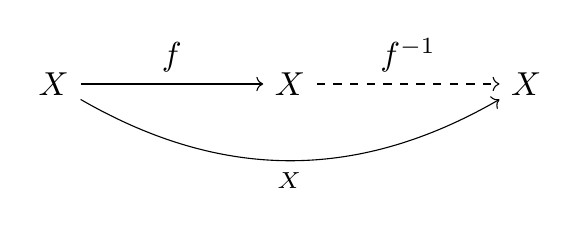
\begin{tikzpicture}[scale=3, nodes={scale=1.2}]
\node (X1)  at (0, 0) {$X$};
\node (X2)  at (1, 0) {$X$};
\node (X3)  at (2, 0) {$X$};

\path[->] (X1) edge             node[above]{$f$}        (X2)
          (X2) edge[dashed]     node[above]{$f^{-1}$}   (X3)
          (X1) edge[bend right] node[below]{$\id_X$}    (X3);
\end{tikzpicture} \qquad 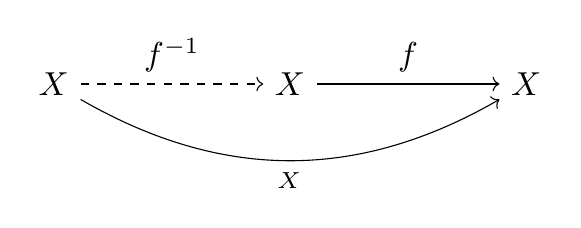
\begin{tikzpicture}[scale=3, nodes={scale=1.2}]
\node (X1)  at (0, 0) {$X$};
\node (X2)  at (1, 0) {$X$};
\node (X3)  at (2, 0) {$X$};

\path[->] (X2) edge             node[above]{$f$}        (X3)
          (X1) edge[dashed]     node[above]{$f^{-1}$}   (X2)
          (X1) edge[bend right] node[below]{$\id_X$}    (X3);
\end{tikzpicture} \]

Additionally, $f \in \aut(X)$ requires that $f \in \sym(X)$ and $f$
preserves whatever structure $X$ has. Suppose $X$ is a group/ring/field.
Then for each operation $*$, we require the following diagram to commute
as well.
\[ 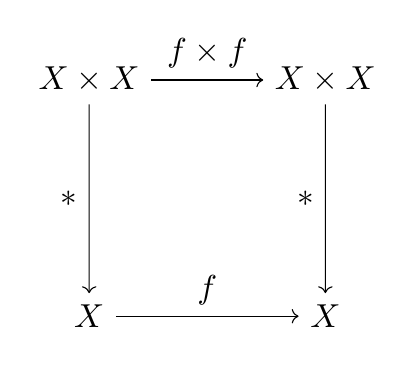
\begin{tikzpicture}[scale=3, nodes={scale=1.2}]
\node (XX1) at (0, 1) {$X \times X$};
\node (XX2) at (1, 1) {$X \times X$};
\node (X1)  at (0, 0) {$X$};
\node (X2)  at (1, 0) {$X$};

\path[->]
(XX1) edge node[above]{$f \times f$}    (XX2)
(XX1) edge node[left] {$*$}             (X1)
(X1)  edge node[above]{$f$}             (X2)
(XX2) edge node[left] {$*$}             (X2);
\end{tikzpicture} \]
\end{note}

Anyways, we now explore what exactly we mean in
definition~\ref{sdprod}. Suppose $N, A$ are two subgroups so that $f : N
\times A \to G, (n, a) \xmapsto{f} na$ is a bijection. This implies that
every element in $g \in G$ can be written uniquely as $g = na, n \in N,
a \in A$.  It also implies that $N \cap A = \lbrace e \rbrace$, because
$g \in N \cap A \implies g = e_N g_A = g_N e_G$ and uniqueness gives $g
= e$. Now suppose further that $N \lhd G$. Then we have $\forall n_1,
n_2 \in N, a_1, a_2 \in A$,
\[ \begin{aligned}
(n_1 a_1)(n_2 a_2) &= n_1 a_1 n_2 a_1^{-1} a_1 a_2 \\
\implies f^{-1}(f(n_1, a_1) \cdot f(n_2, a_2)) &= (n_1 (a_1 n_2
a_1^{-1}), a_1 a_2) \\
\implies f(n_1, a_1) \cdot f(n_2, a_2) &= f(n_1 (a_1 n_2 a_1^{-1}), a_1
a_2), \\
\end{aligned} \]
so $f$ is a isomorphism only if we define the multiplication on $N
\times A$ to be $(n_1, a_1)(n_2, a_2) = (n_1 (a_1 n_2 a_1^{-1}), a_1
a_2)$.

$N$ is also normal in $G$ so we can say that $A$ acts on $N$ by
conjugation.

\section{October 14, 2015}

\subsection{Review}
Last time, we saw that given $K, N \leq G, N \lhd G$ and $f : N \times K
\to G, (n, k) \mapsto nk$ is a bijection, we can define a multiplication
on $N \times K$ so that $f$ is a homomorphism.

\begin{lem}
Let $N \lhd G, K \leq G$. Then $NK = \lbrace nk \mid n \in N, k \in G
\rbrace$ is a subgroup of $G$.
\end{lem}

\begin{proof}
We want $(n_1 k_1)(n_2 k_2)^{-1} \in NK$, so we compute
\[ (n_1 k_1)(n_2 k_2) = n_1 k_1 k_2^{-1} n_2^{-1} = n_1 (k_1 k_2^{-1})
n_2^{-1} (k_1 k_2^{-1})^{-1} (k_1 k_2^{-1}) = n_1 n_3 k_3 \in NK. \]
\end{proof}

\subsection{More Semidirect Products}
Recall that $\rho : K \to \aut(N)$ gives an action of $K$ on $N$, namely
$k \cdot n = \rho(k)(n)$. Moreover, $k \cdot (n_1 n_2) = \rho(k)(n_1
n_2) = \rho(k)(n_1) \rho(k)(n_2) = (k \cdot n_1)(k \cdot n_2)$.

\begin{thm}
\label{externalsemiprod}
Let $K, N$ be two groups, $\rho : K \to \aut(N)$ a homomorphism and $K
\times N \to N, k \cdot n = \rho(k)(n)$ be the corresponding action.
Then the operation $* : (N \times K) \times (N \times K) \to N \times K$
given by $(n_1, k_1) * (n_2, k_2) = (n_1 (k_1 \cdot n_2)), k_1 k_2)$ is
an associative binary operation that turns $N \times K$ into a group.
This group is denoted $N \rtimes_\rho K$.
\end{thm}

\begin{proof}
Trivial.
\end{proof}

\begin{note}
At this point, I would like to distinguish between \textbf{internal
semidirect products} and \textbf{external semidirect products}. An
internal product is formed when we take some group and form a semidirect
product structure out of subgroups, while an external product has the
notion of taking two completely unrelated groups (except by action via
group automorphisms), and forming a new group. More preciselly,
splitting $G \to N \rtimes K$ would be forming an internal product while
combining $N, K \to N \rtimes K$ would be forming an external product.
\end{note}

\begin{ex}
$\RR^{\times}$ acts on $\RR$ by isomorphisms given by multiplication,
and we have the properties $a \cdot b = ab, a(b + c) = ab + ac$. By
\ref{externalsemiprod}, we get that $\RR \rtimes \RR^\times$ is a group
with multiplication $(b, a) * (b', a') = (b + ab', aa')$. We claim that
$\RR \rtimes \RR^\times \iso \aff(\RR)$.
\end{ex}

\begin{proof}[Reason]
Consider $\varphi : \RR \rtimes \RR^\times \to \aff(\RR)$ given by $(b, a)
\mapsto \lbrace x \mapsto ax + b \rbrace$. Now compute
\[ \begin{aligned}
(\varphi(b, a) \circ \varphi(b', a'))(x) &= \varphi(b, a)(a'x + b') \\
&= a(a'x + b') + b \\
&= b + ab' + aa'x \\
&= \varphi((b, a) * (b', a'))(x) \\
\end{aligned} \]
\end{proof}

\begin{rem}
$\widetilde{N} = N \times \lbrace e \rbrace \iso N$ and $\widetilde{K} =
\lbrace e \rbrace \times K \iso K$. The action of $\widetilde{K}$ on
$\widetilde{N}$ by conjugation recovers the action of $K$ on $N$.
\end{rem}

\begin{ex}
If $G$ is abelian, then the inverse map $g \mapsto g^{-1}$ is trivially
an isomorphism, which gives that there is some map $\ZZ / 2 \ZZ
\xrightarrow{\rho} \aut(G)$ with $\rho([1]) = \lbrace g \mapsto g^{-1}
\rbrace$ gives us a semidirect product $G \rtimes_\rho \ZZ / 2 \ZZ$.
Taking $G = \ZZ / n \ZZ$, we trivially get $\ZZ / n \ZZ \rtimes_\rho \ZZ
/ 2 \ZZ \iso D_{2n}$.
\end{ex}

\section{October 19, 2015}

\section{October 19, 2015}

\section{October 23, 2015}

\subsection{Review}

\begin{rem}
We have some interesting trivial corollaries from ideals.
\begin{enumerate}
\item $1 \in I \implies I = R$.
\item $u \in R^\times, u \in I \implies I = R$.
\item If $F$ is a field, the only ideals are $0, F$.
\end{enumerate}
\end{rem}

\subsection{Quotient Rings and The First Isomorphism Theorem (again)}
\begin{thm}
Let $I$ be an ideal of some ring $R$. Then
\begin{enumerate}
\item The \textbf{quotient group} $R / I = \lbrace a + I \mid a \in R
\rbrace$ is a ring with multiplication given by $(a + I)(b + I) = ab +
I$.
\item $\pi : R \to R / I$ is a ring homomorphism.
\item $1 \mapsto 1 + I = 1_{R / I}$.
\end{enumerate}
$R / I$ is now known as the \textbf{quotient ring} of $R$ mod $I$.
\end{thm}

\begin{proof}
Trivial.
\end{proof}

\begin{prop}
If $\varphi : R \to R'$ is a ring homomorphism, then $\varphi(R)$ is a
subring of $R'$.
\end{prop}

\begin{thm}[First Isomorphism Theorem]
Let $\varphi : R \to R'$ be a ring homomorphism. Then there exists a
unique ring homomorphism $\overline{\varphi} : R / \ker \varphi \to R'$
given by $r + I \xmapsto{\overline{\varphi}} \varphi(r)$.
\end{thm}

\begin{proof}
We easiliy get that $R / \ker\varphi \to R'$ is a well defined group
homomorphism, so we only need to check it for multiplication. But this
is easy because
\[ \overline{\varphi}((a + I)(b + I)) = \overline{\varphi}(ab + I) =
\varphi(ab) = \varphi(a)\varphi(b) = \overline{\varphi}(a + I)
\overline{\varphi}(b + I). \]
\end{proof}

\begin{ex}
Canonical inclusion $\iota : \RR \to \CC$ is a ring homomorphism, so we
get some $f : \RR[X] \to \CC$ with $X \mapsto \sqrt{-1}$. In particular,
\[ \sum_{j = 0}^n a_j X^j = \sum_{j = 0}^n a_j (\sqrt{-1})^j. \]
Trivially, $\ker f = (X^2 + 1)\RR[X]$.
\end{ex}

\subsection{Generating Ideals}
Similarly to generating subgroups from a set of elements, we can also
generate ideals. Namely,
\[ \bigcap_{I \in A} I = \lbrace i \mid i \in I \quad \forall I \in A
\rbrace \]
for some set of ideals $A$ is also an ideal. Now let $A$ be the set of
ideals all containing some ideal $S$. Then $\cycgroup{S}$ is the
smallest ideal containing $S$.

\begin{df}
$\cycgroup{\lbrace a \rbrace} = \lbrace ar \mid r \in R \rbrace = aR$ is
called the \textbf{principal ideal} generated by $a$.
\end{df}

\section{October 23, 2015}

\subsection{Review}

\begin{rem}
We have some interesting trivial corollaries from ideals.
\begin{enumerate}
\item $1 \in I \implies I = R$.
\item $u \in R^\times, u \in I \implies I = R$.
\item If $F$ is a field, the only ideals are $0, F$.
\end{enumerate}
\end{rem}

\subsection{Quotient Rings and The First Isomorphism Theorem (again)}
\begin{thm}
Let $I$ be an ideal of some ring $R$. Then
\begin{enumerate}
\item The \textbf{quotient group} $R / I = \lbrace a + I \mid a \in R
\rbrace$ is a ring with multiplication given by $(a + I)(b + I) = ab +
I$.
\item $\pi : R \to R / I$ is a ring homomorphism.
\item $1 \mapsto 1 + I = 1_{R / I}$.
\end{enumerate}
$R / I$ is now known as the \textbf{quotient ring} of $R$ mod $I$.
\end{thm}

\begin{proof}
Trivial.
\end{proof}

\begin{prop}
If $\varphi : R \to R'$ is a ring homomorphism, then $\varphi(R)$ is a
subring of $R'$.
\end{prop}

\begin{thm}[First Isomorphism Theorem]
Let $\varphi : R \to R'$ be a ring homomorphism. Then there exists a
unique ring homomorphism $\overline{\varphi} : R / \ker \varphi \to R'$
given by $r + I \xmapsto{\overline{\varphi}} \varphi(r)$.
\end{thm}

\begin{proof}
We easiliy get that $R / \ker\varphi \to R'$ is a well defined group
homomorphism, so we only need to check it for multiplication. But this
is easy because
\[ \overline{\varphi}((a + I)(b + I)) = \overline{\varphi}(ab + I) =
\varphi(ab) = \varphi(a)\varphi(b) = \overline{\varphi}(a + I)
\overline{\varphi}(b + I). \]
\end{proof}

\begin{ex}
Canonical inclusion $\iota : \RR \to \CC$ is a ring homomorphism, so we
get some $f : \RR[X] \to \CC$ with $X \mapsto \sqrt{-1}$. In particular,
\[ \sum_{j = 0}^n a_j X^j = \sum_{j = 0}^n a_j (\sqrt{-1})^j. \]
Trivially, $\ker f = (X^2 + 1)\RR[X]$.
\end{ex}

\subsection{Generating Ideals}
Similarly to generating subgroups from a set of elements, we can also
generate ideals. Namely,
\[ \bigcap_{I \in A} I = \lbrace i \mid i \in I \quad \forall I \in A
\rbrace \]
for some set of ideals $A$ is also an ideal. Now let $A$ be the set of
ideals all containing some ideal $S$. Then $\cycgroup{S}$ is the
smallest ideal containing $S$.

\begin{df}
$\cycgroup{\lbrace a \rbrace} = \lbrace ar \mid r \in R \rbrace = aR$ is
called the \textbf{principal ideal} generated by $a$.
\end{df}

\section{October 26, 2015}

\subsection{Integral Domains}

\begin{df}
Let $R$ be a ring, $b \in R, b \neq 0$. $b$ is called a \textbf{zero
divisor} if $\exists a \in R, a \neq 0 \st ab = 0$ or $ba = 0$.
\end{df}

\begin{ex}
We have $\begin{pmatrix} 0 & 1 \\ 0 & 0 \end{pmatrix}$ as a zero divisor
of itself in $GL_2(\RR)$.
\end{ex}

\begin{ex}
$2 \cdot 3 = 0$ in $\ZZ / 6 \ZZ$.
\end{ex}

\begin{prop}
Zero divisors cannot be units and units cannot be zero divisors.
\end{prop}

\begin{proof}
Suppose $d \in $ is a unit and zero divisor. Then $\exists b \in R \st b
\neq 0, db = 0$. Also $\exists u \in R \st ud = 1$. Then compute
\[ 0 = u \cdot 0 = u \cdot (db) = (ud)b = 1 \cdot b = b \]
to get a contradiction.
\end{proof}

\begin{rem}
Fields have no zero divisors. Consequently, any subring of a field has
no zero divisors.
\end{rem}

\begin{df}
A commutative ring with identity and no zero divisors is called an
\textbf{integral domain}.
\end{df}

\begin{prop}
Suppose $R$ is a ring with $a, b, c \in R$, $a \neq 0$ is not a zero
divisor. Then
\[ ab = ac \implies b = c. \]
\end{prop}

\begin{proof}
Rewrite as
\[ ab - ac = 0 \implies a(b - c) = 0 \implies b - c = 0 \implies b = c.
\]
\end{proof}

\begin{rem}
This forms the basis for the \textbf{cancellation law} in integral
domains.
\end{rem}

\begin{rem}
$\ZZ / n \ZZ$ is an integral domain $\iff$ $n$ is prime.
\end{rem}

\begin{prop}
Any finite integral domain is a field.
\end{prop}

\begin{proof}
Let $D$ be a finite integral domain, $a \in D, a \neq 0$. We want to
find an $x \in D$ such that $ax = 1$. Instead, we show that the map $L_a
: D \surj D, x \xmapsto{L_a} ax$ is surjective. By cancellation, we have
that $L_a(b) = L_a(c) \implies b = c$ so $L_a : D \inj D$ is injective.
$D$ is finite so $D$ is also surjective.
\end{proof}

\begin{prop}
Let $D$ be an integral domain. Then for all $f, g \in D[X]$, we have
\[ \deg(fg) = \deg f + \deg g. \]
\end{prop}

\begin{proof}
Suppose $f, g \neq 0$. $\deg f = n \geq 0, \deg g = m \geq 0$. Then
perform polynomial multiplication. Namely,
\[ (a_0 + \cdots + a_n X^n)(b_1 + \cdots b_mX^m) = c_0 + \cdots + a_n
b_m X^{n + m} \]
and $a_n b_m \neq 0$.
\end{proof}

\begin{cor}
$D[X]$ is integral if $D$ is integral.
\end{cor}

\subsection{More Ideals}

\begin{ex}
$\cycgroup{2, x}$ is not principal in $\ZZ[x]$.
\end{ex}

\begin{proof}
Suppose $\cycgroup{2, x} = \cycgroup{a(x)}$ for some $a(x) \in \ZZ[x]$.
Then $2 = a(x) q(x)$ for some $q(x) \in \ZZ[x]$ so
\[ 0 = \deg 2 = \deg a(x) + \deg q(x) \implies a(x) = a \in \ZZ \quad
q(x) = q \in \ZZ \implies 2 = aq \implies a = \pm 1, \pm 2. \]
However, $\pm 1 \not \in \cycgroup{2, x}$ so $a = \pm 2$. This means
that $\exists r(x) \in \ZZ[x]$ such that $x = 2 \cdot r(x)$ so $r(x) =
b_0 + b_1 x$ for some $b_0, b_1$ and $2r(x) = 2b_0 + 2b_1 x \implies b_0
= 0, 1 = 2b_1$ but then $b_1$ is not an integer.
\end{proof}

\section{October 28, 2015}

\subsection{Polynomial Rings Over Fields are Euclidean}

\begin{thm}
Let $F$ be a field with $f, d \in F[X]$ and $g \neq 0$. Then $\exists !$
$q, r \in F[X]$ such that
\begin{enumerate}
\item $f = qd + r$.
\item $\deg r < \deg d$.
\end{enumerate}
\end{thm}

\begin{proof}
Existence is easy. If $\deg f > \deg d$, then $f = 0d + f$, so we now
suppose that $\deg f \geq \deg d$ and induct on $n$. If $n = 0$, then $f
= c_1 \in F, d = c_2 \in F, c_2 \neq 0$, and $c_1 = \left(b_0
a_0^{-1}\right) a_0 + 0$. so it holds for $n = 0$. Now assume it holds
for all $c, d \in F[X]$ with $\deg c < n$.
\end{proof}

\section{October 28, 2015}

\section{October 28, 2015}

\section{October 28, 2015}

\section{October 28, 2015}

\section{October 28, 2015}


\end{document}
